\fakesection{Classification}{\hfill\small\texttt{/src/session\_1/.m}}

\begingroup
\setlength{\columnsep}{0.75cm}
\setlength{\intextsep}{1cm}
\begin{wrapfigure}{r}{0pt}
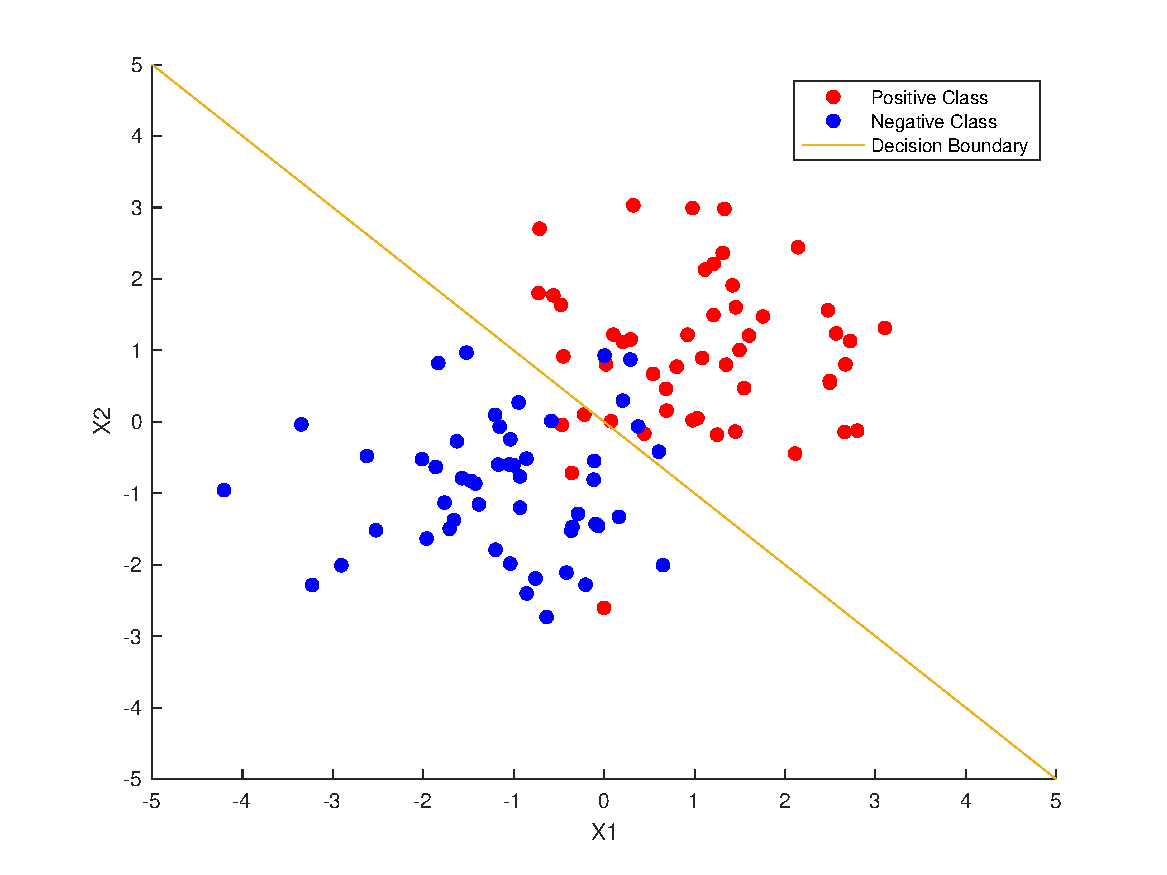
\includegraphics[width=0.5\textwidth]{../src/figures/twogaussians.pdf}
\caption{Decision boundary for two Gaussian distributions with equal covariance matrices.}
\label{twogaussians}
\end{wrapfigure}
\fakesubsection{Two Gaussians}{}
For a binary classifier where the distributions are (assumed or known to be) Gaussian with equal covariance matrices the decision boundary that maximises the posterior probability $P(C_i|x)$ becomes linear. This is independent of the amount of overlap. Trying to get a better boundary would lead to overfitting. In this particular example where $\Sigma_{xx}=\mathbb{I}$ one ends up with a perpendicular bisector of the segment connecting the two cluster means 
$(-1,-1)$ and $(1,1)$, which gives $f(x)=-x$ as a decision boundary.
\fakesubsection{Support Vector Machine Classifier}{}
To deal with the non-linearly separable classification problem in the example one solves the following minimisation problem, where the hyperparameter $C$ controls the tradeoff between maximising the margin and making sure that the data lies on the correct side of that margin :

\endgroup

$$\min_x\frac{1}{2}\cdot w^T\cdot w+C\cdot \sum_{k=1}^N\xi_k\qquad\text{such that $y_k\cdot[w^T\cdot x_k+b]\geq 1-\xi_k$ and $\xi_k\geq 0$ $(\forall k\in\{1,..,N\})$}$$
A dual form can be expressed by making use of Lagrange multipliers which in this context are also called \textit{support values}. Any data points for which the corresponding support value isn't zero are called \textit{support vectors}. These lie close to the boundary or are misclassified.

\par\noindent For the given toy dataset it can readily be seen in figure \ref{stanfordexample} (top row) that for a decreasing value of $C$ the margin does become larger and that less \textit{`slacking'} is allowed for. By adding data points close to the boundary or at the \textit{`wrong'} side of it the margin usually changes a lot and the new data points nearly always become support vectors.

\begin{figure}[h]
\centering
\subfloat[$C = 0.01$ (large margin, lots of \textit{`slacking'}.)]{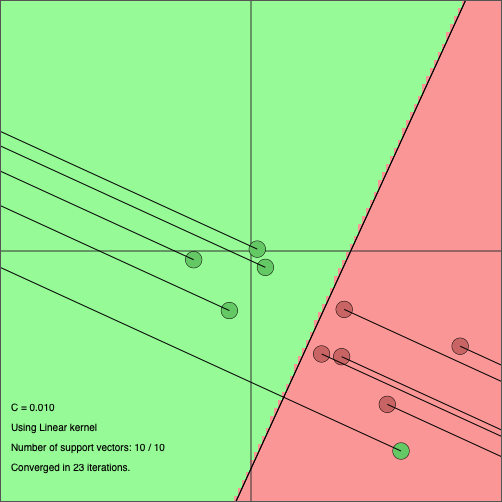
\includegraphics[width=0.17\textwidth]{../src/figures/stanford/canvas01}}\qquad
\subfloat[$C = 1$]{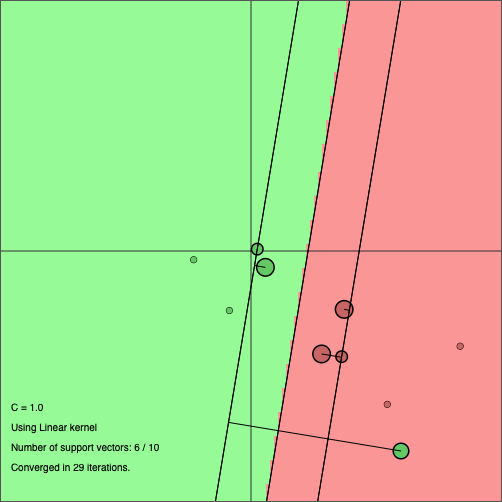
\includegraphics[width=0.17\textwidth]{../src/figures/stanford/canvas1}}\qquad
\subfloat[$C = 10$ (small margin, little \textit{`slacking'}.]{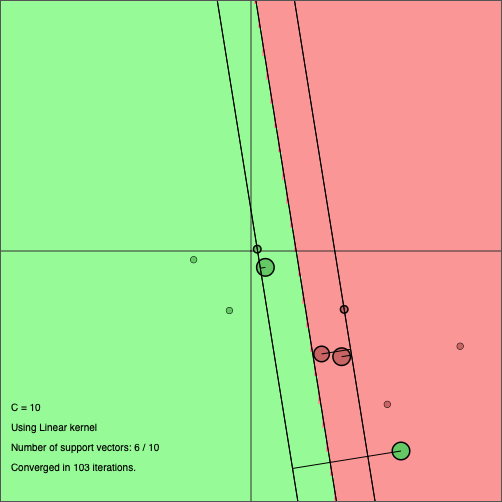
\includegraphics[width=0.17\textwidth]{../src/figures/stanford/canvas10}}\\
\subfloat[Initial solution.]{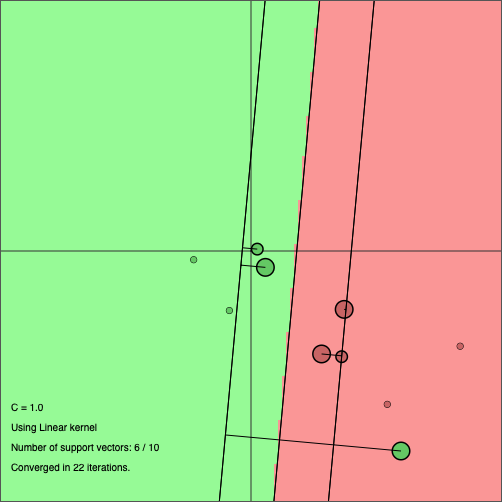
\includegraphics[width=0.17\textwidth]{../src/figures/stanford/canvasnew}}\qquad
\subfloat[Negative data points added at the right side of the margin.]{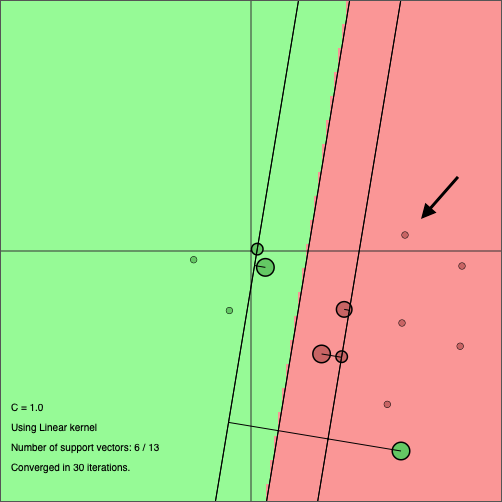
\includegraphics[width=0.17\textwidth]{../src/figures/stanford/canvasnew2}}\qquad
\subfloat[Negative data point added at the other side of the margin.]{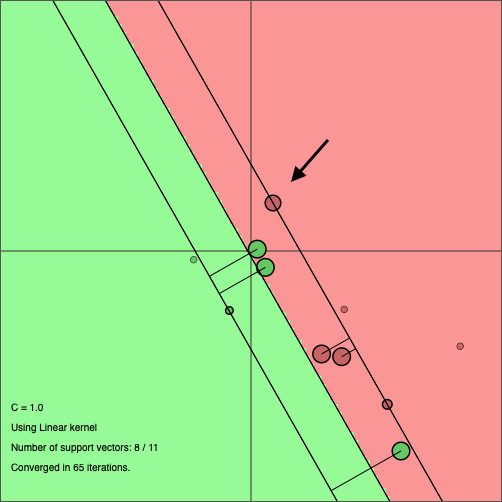
\includegraphics[width=0.17\textwidth]{../src/figures/stanford/canvasnew3}}\\
\subfloat[$\sigma=0.1$]{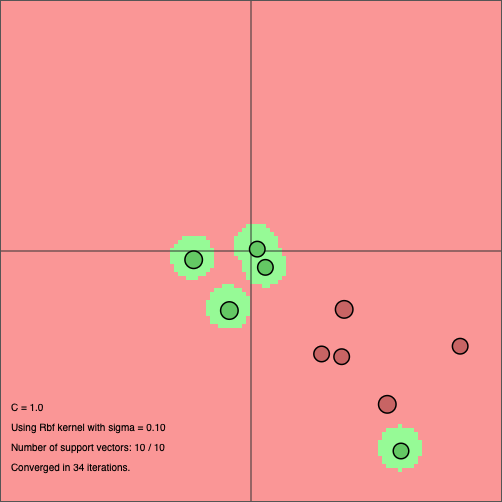
\includegraphics[width=0.17\textwidth]{../src/figures/stanford/canvasrbf025}}\qquad
\subfloat[$\sigma=1.0$]{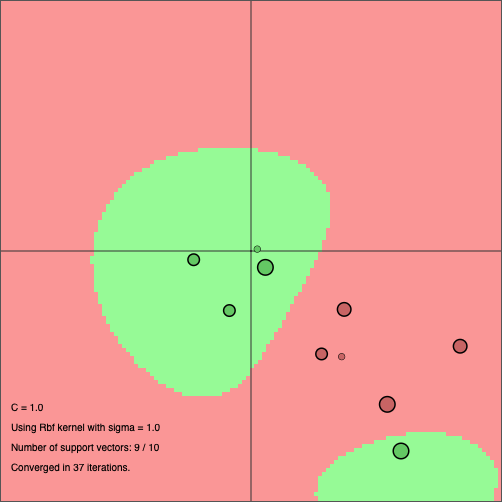
\includegraphics[width=0.17\textwidth]{../src/figures/stanford/canvasrbf1}}\qquad
\subfloat[$\sigma=100$]{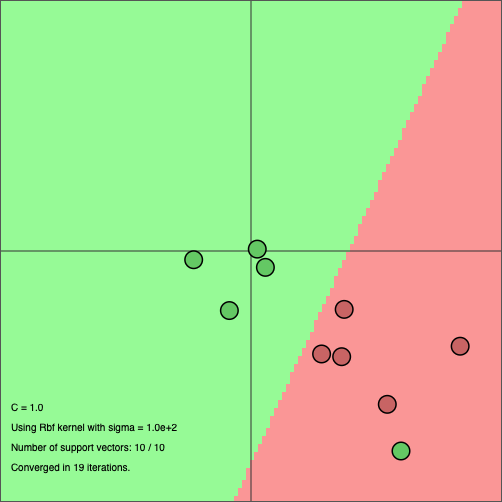
\includegraphics[width=0.17\textwidth]{../src/figures/stanford/canvasrbf100}}\\
\subfloat[Negative data point added far away from the boundary.]{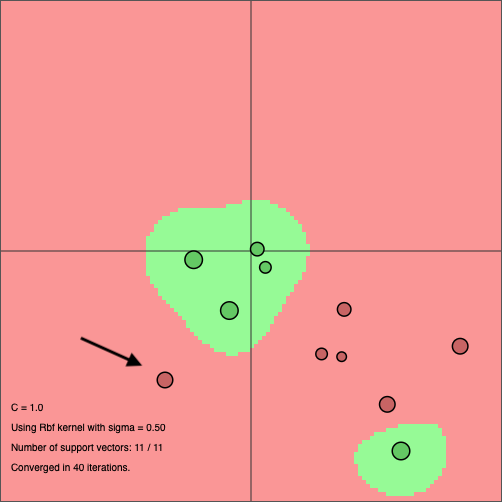
\includegraphics[width=0.17\textwidth]{../src/figures/stanford/canvasnewrbf1}}\qquad
\subfloat[Positive data point added inside the boundary.]{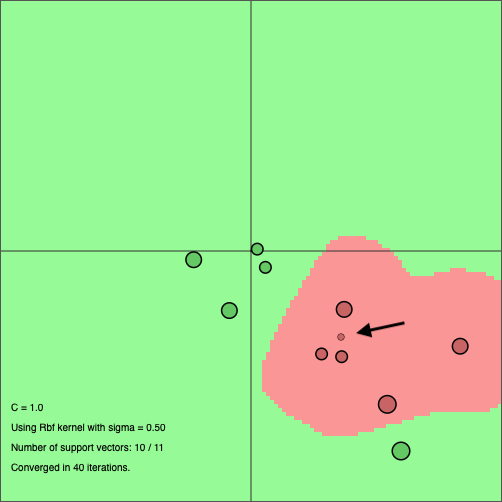
\includegraphics[width=0.17\textwidth]{../src/figures/stanford/canvasnewrbf2}}\qquad
\subfloat[Positive data point added inside the boundary.]{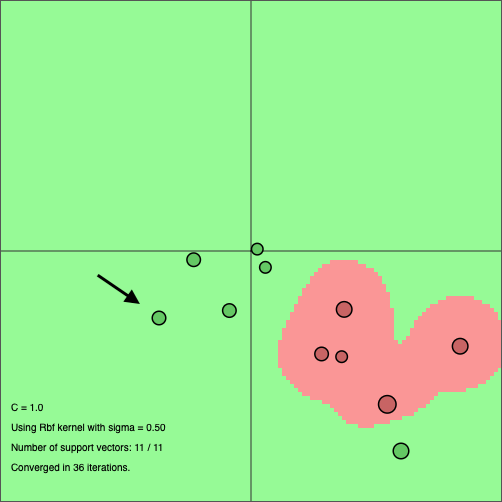
\includegraphics[width=0.17\textwidth]{../src/figures/stanford/canvasnewrbf3}}
\caption{Visualisation of various experiments with $C$ (top row), addition of points using the linear kernel (second row), $\sigma$ (third row) and addition of points using the RBF kernel (last row). The number of iterations (tends to) increase as $C$ gets larger or as the number of data points increases.}
\label{stanfordexample}
\end{figure}

\noindent The $\sigma$ hyperparameter in the case of an RBF kernel controls the locality of each data point. As it increases the feature space mapping becomes smoother, producing simpler decision boundaries (figure \ref{stanfordexample}, third row). This relates to the bias-variance tradeoff. For very large bandwidths the peaks around the data points are flattened out and linear separation in the feature space isn't possible anymore which may lead to a result similar to the linear kernel or may even lead to one class overtaking the other. As for $C$, it works the same as before, prioritising either larger margins or lower misclassification rates. When $\sigma$ is large a bigger value of $C$ can make the model more complex again. 

\par\noindent The RBF kernel approach can generate models having misclassification rates that are lower than the classic linear kernel approach does as decision boundaries that are nonlinear in the input space can be learned. It also uses more data points as support vectors. This makes the model less compact (computationally efficient) and if the data is linearly separable it is unnecessary. Deciding whether the model generalises better can be done through evaluation on a test set.

\fakesubsection{Least-squares support vector machine classifier}{}

Figure \ref{iris} depicts results with various polynomial kernels where $t=1$. This $t$ is called the \textit{constant} and it controls the importance of higher - versus lower-order terms in the polynomial as can be deduced when by applying the binomial theorem on the definition of the kernel :
$$(x^T\cdot y+\tau)^d=\sum_{i=0}^d\binom{d}{i}(x^T\cdot y)^{d-i}\cdot \tau^i$$
The effect of $t$ is not very noticeable for small values of $d$ while for the higher degrees it tends to make the decision boundary more complex.

\par\noindent When the degree $\delta$ is 1 the feature map is linear which is equivalent to the classic non-linear SVM problem while for higher degrees a boundary of increasing complexity is learned such that for $\delta\in\{3,4\}$ no data points are misclassified. To make it less likely that the model overfits a lower $\delta$ is likely to be preferable (which corresponds to Occam's razor).

%\begin{figure}[h]
%\centering
%\subfloat[$\gamma=0.1,\delta=1,\rho=0.5$]{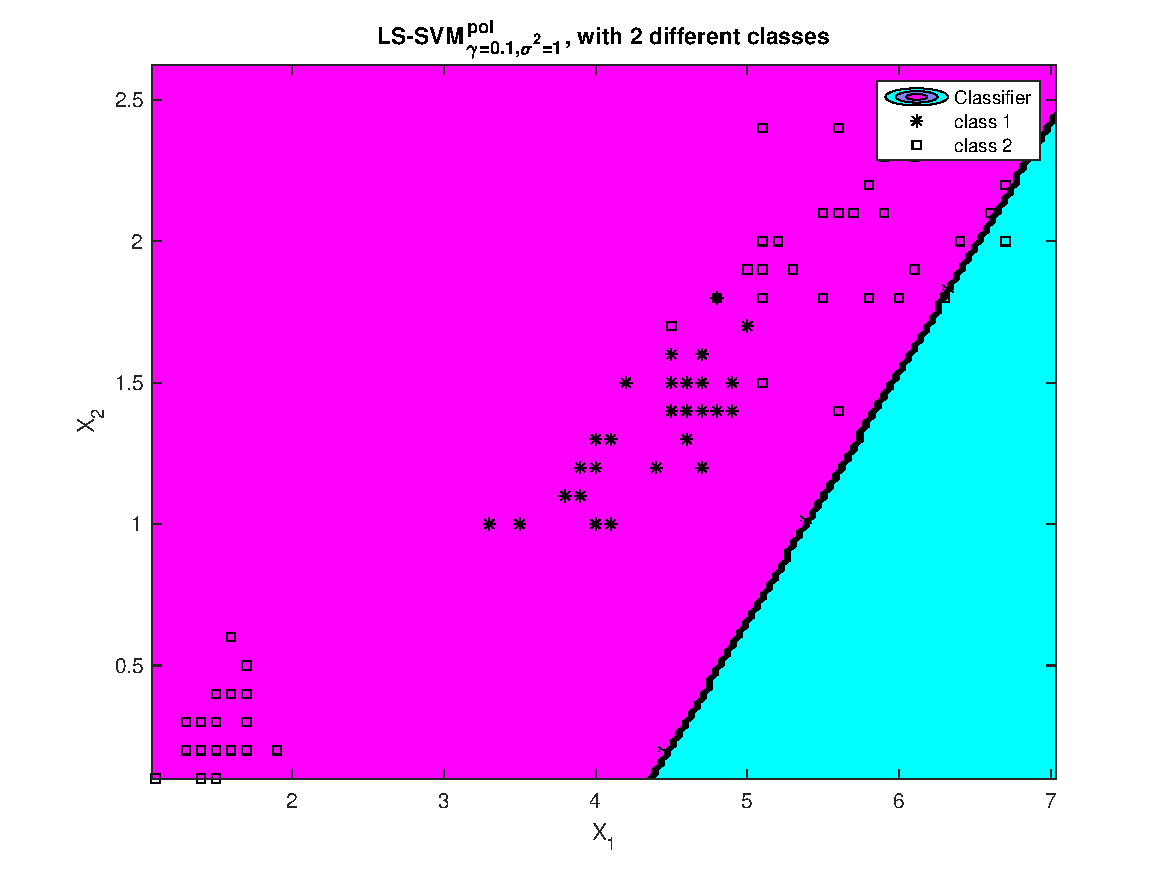
\includegraphics[width=0.3\textwidth]{../src/figures/iris/t=1/1_1}}\qquad
%\subfloat[$\gamma=1.0,\delta=1,\rho=0.55$]{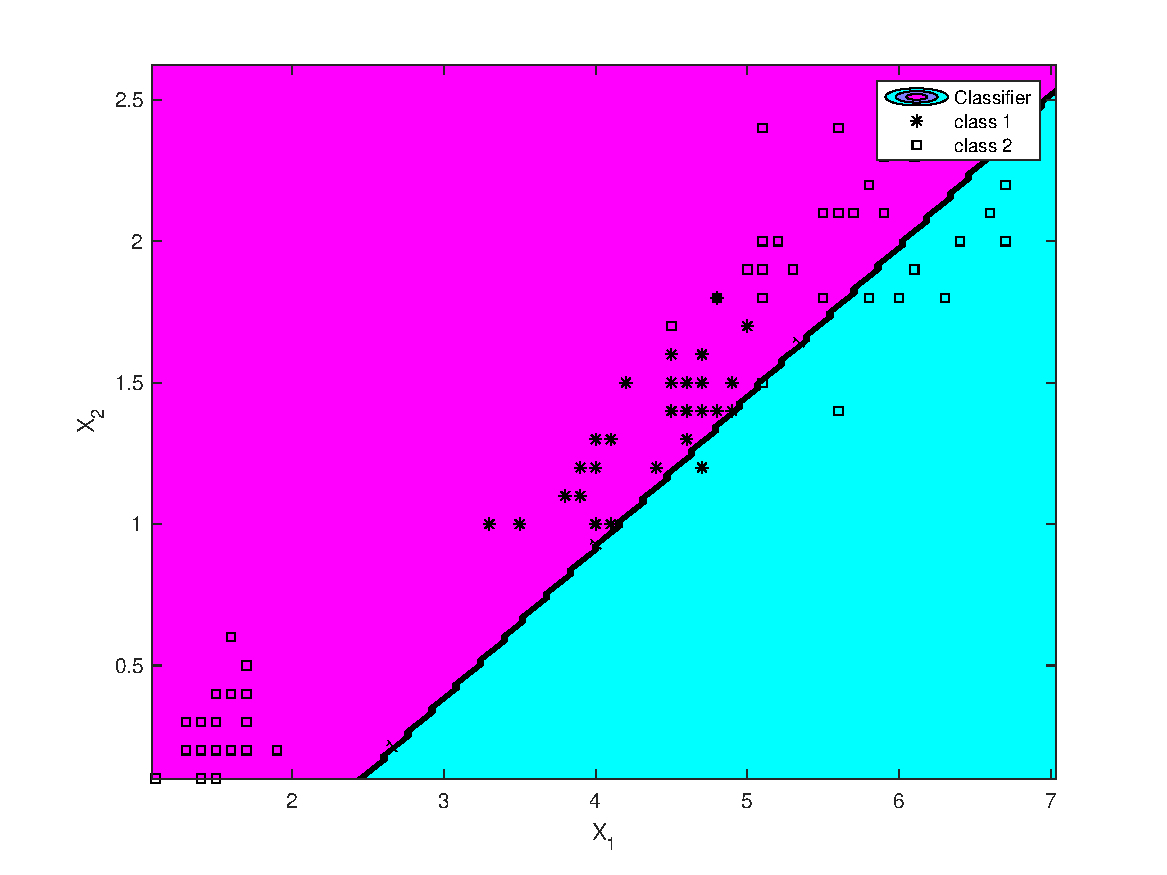
\includegraphics[width=0.3\textwidth]{../src/figures/iris/t=1/1_10}}\qquad
%\subfloat[$\gamma=10.0,\delta=1,\rho=0.55$]{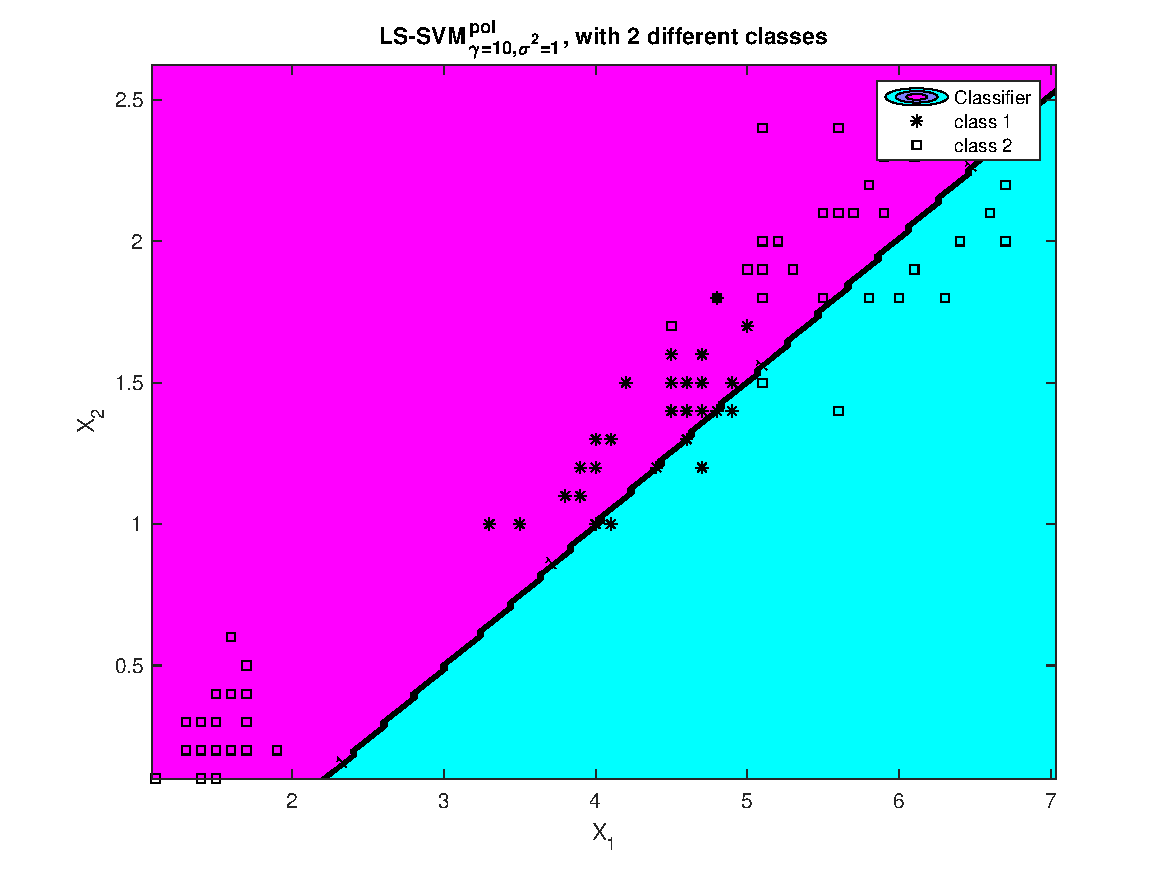
\includegraphics[width=0.3\textwidth]{../src/figures/iris/t=1/1_100}}\qquad
%\\
%\subfloat[$\gamma=0.1,\delta=2,\rho=0.05$]{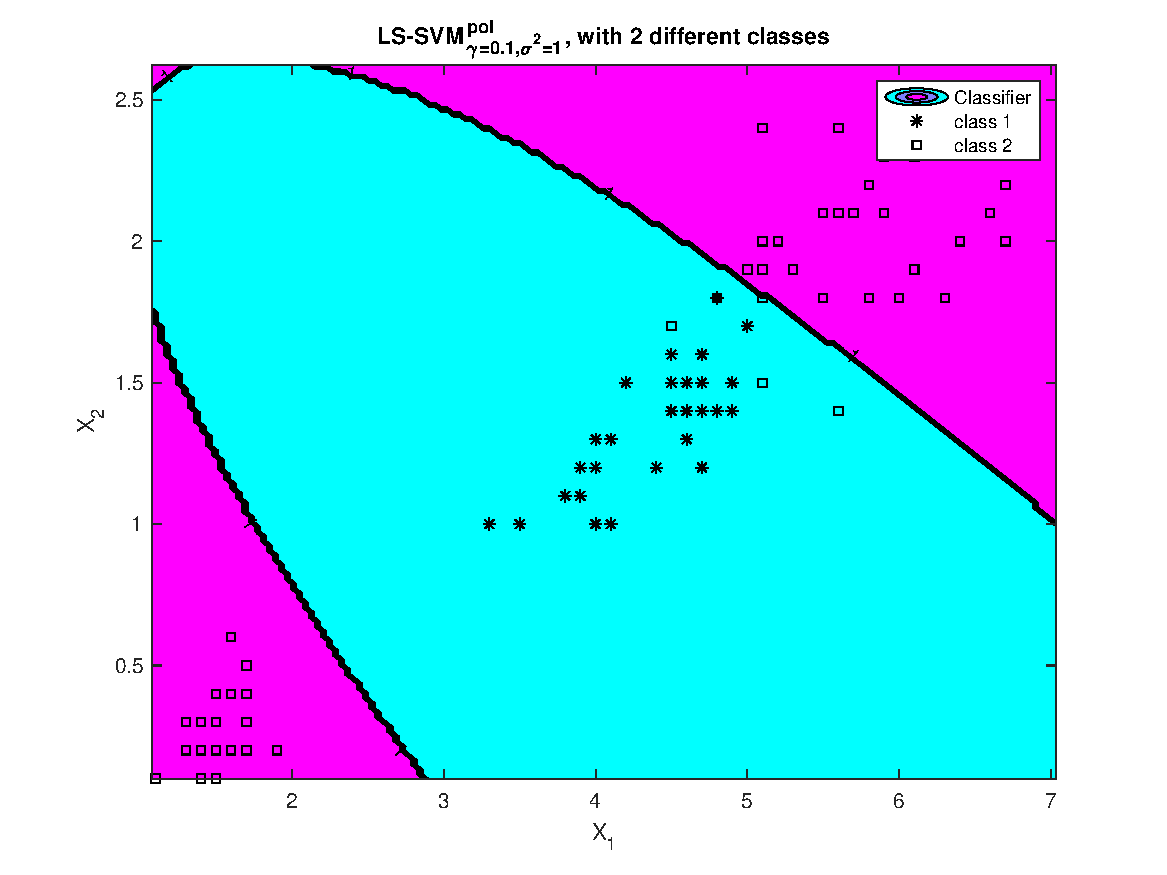
\includegraphics[width=0.3\textwidth]{../src/figures/iris/t=1/2_1}}\qquad
%\subfloat[$\gamma=1.0,\delta=2,\rho=0.05$]{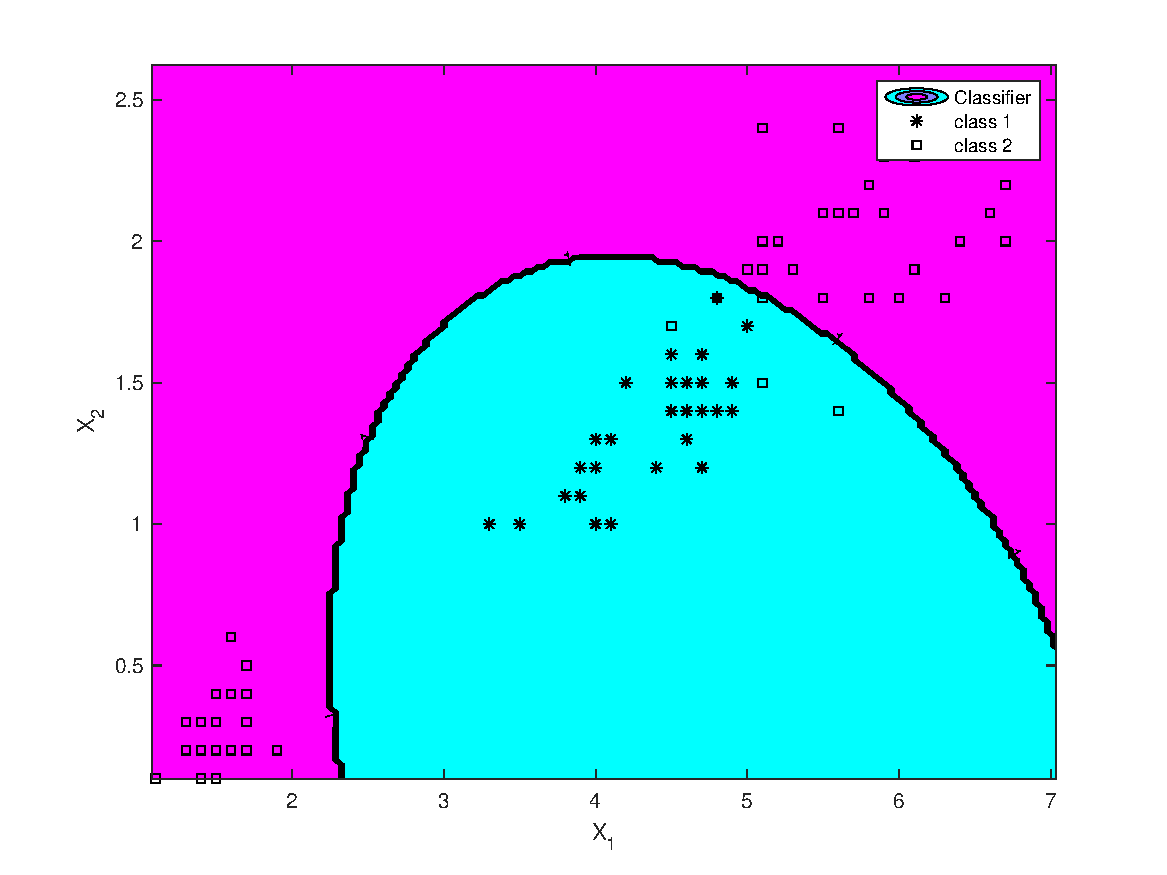
\includegraphics[width=0.3\textwidth]{../src/figures/iris/t=1/2_10}}\qquad
%\subfloat[$\gamma=10.0,\delta=2,\rho=0.05$]{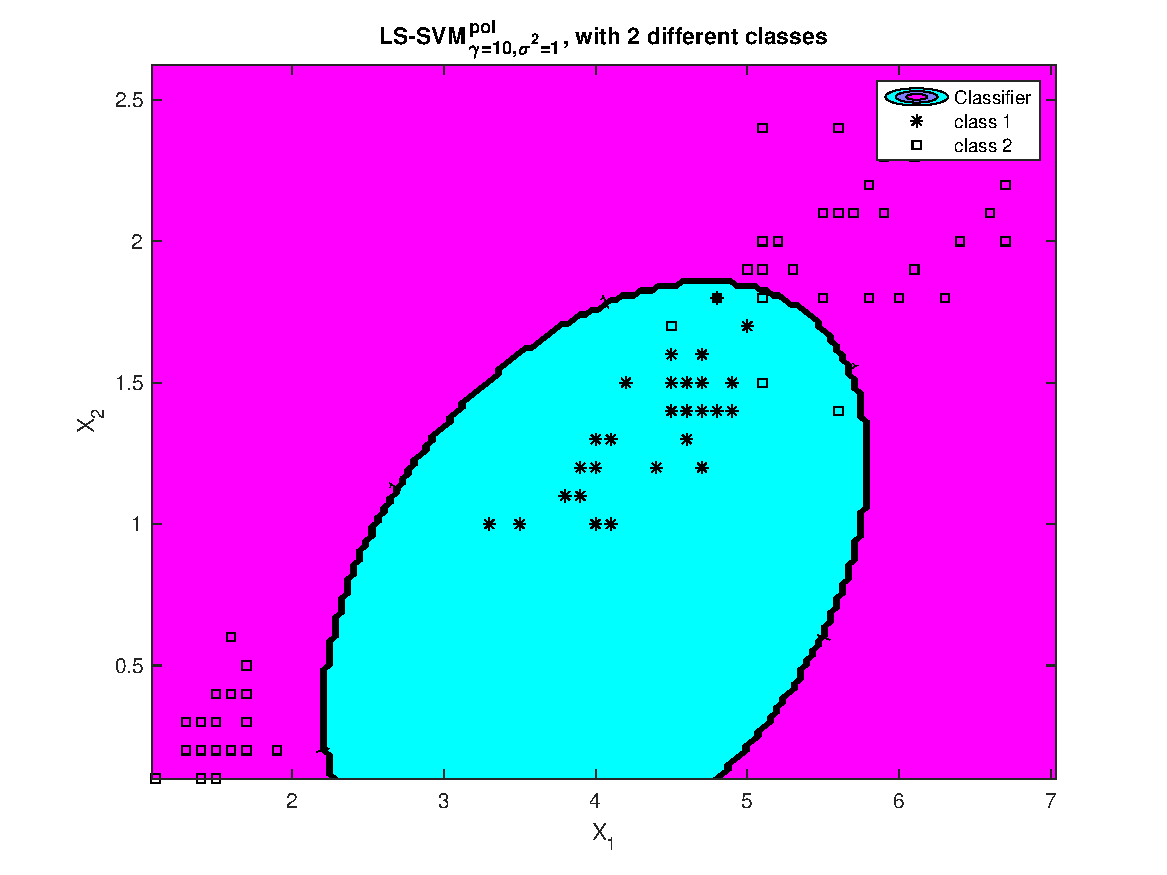
\includegraphics[width=0.3\textwidth]{../src/figures/iris/t=1/2_100}}\qquad
%\\
%\subfloat[$\gamma=0.1,\delta=3,\rho=0.0$]{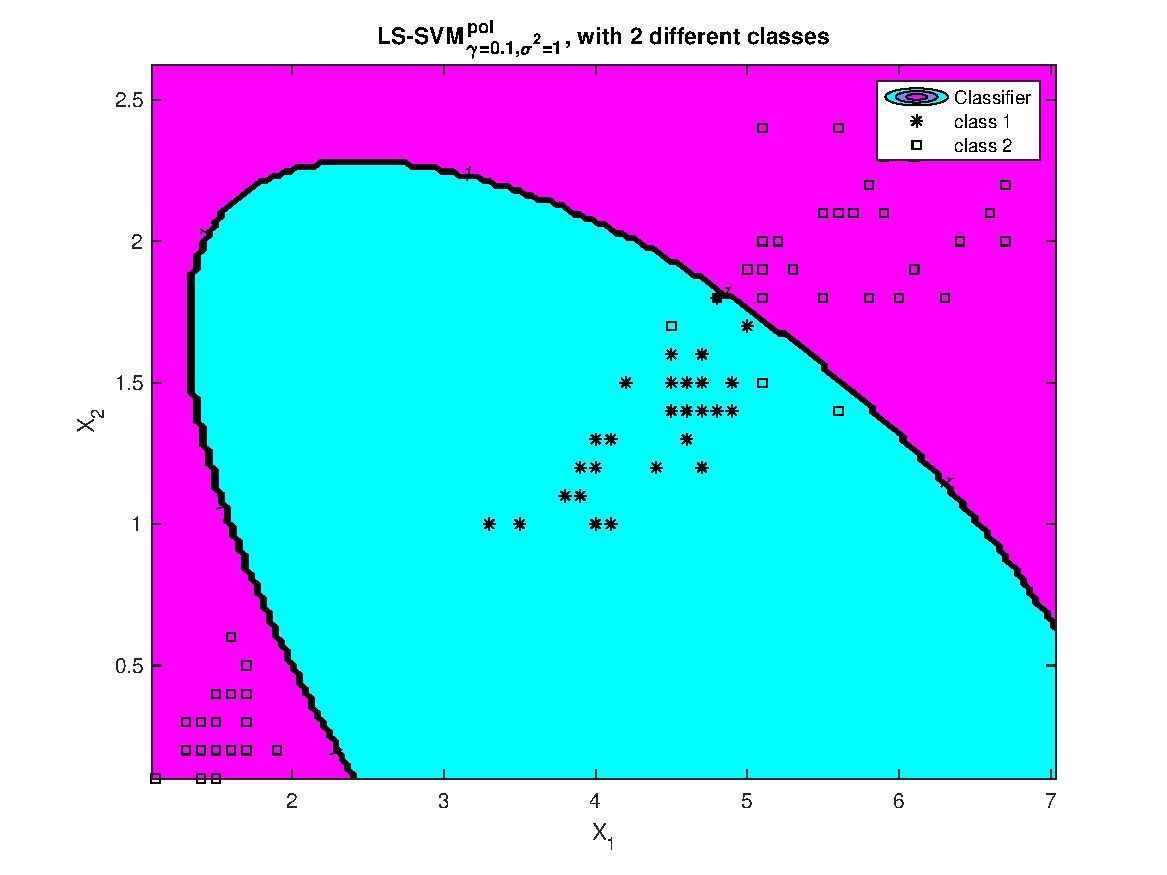
\includegraphics[width=0.3\textwidth]{../src/figures/iris/t=1/3_1}}\qquad
%\subfloat[$\gamma=1.0,\delta=3,\rho=0.0$]{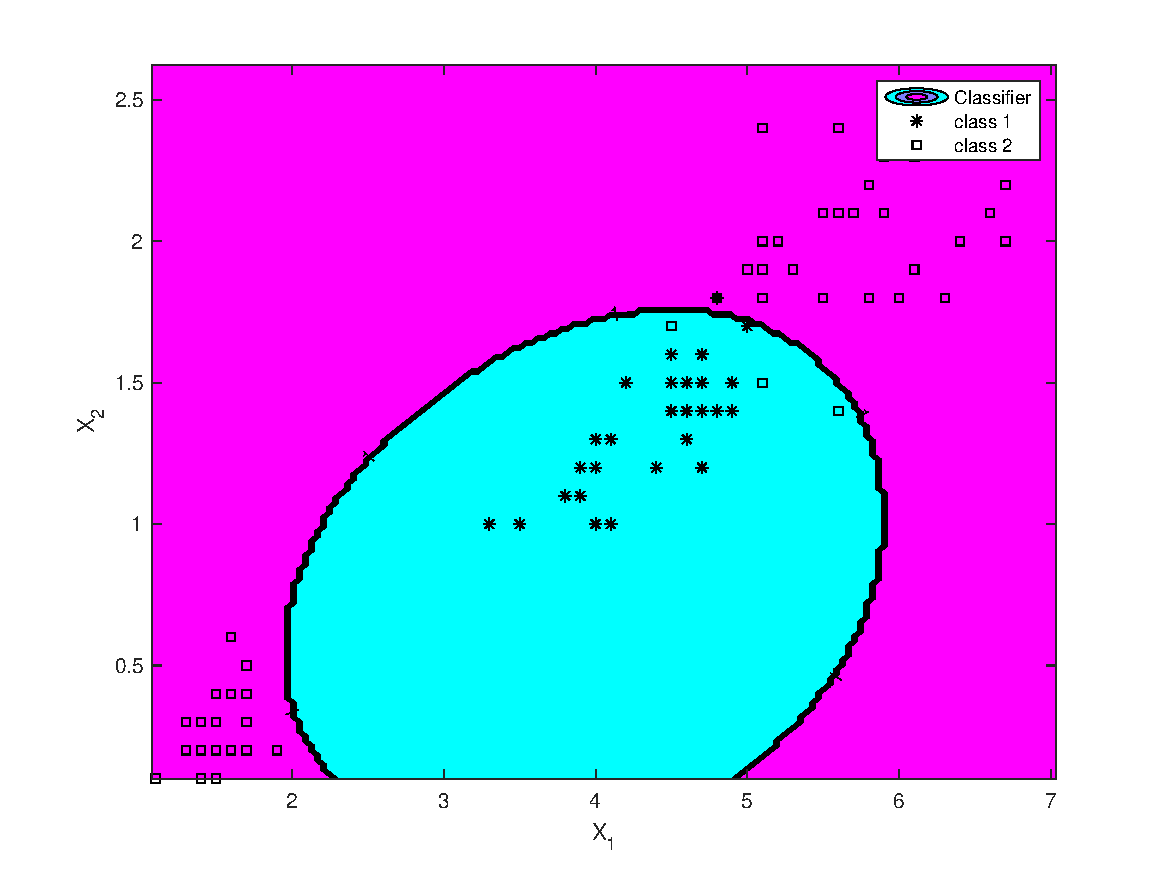
\includegraphics[width=0.3\textwidth]{../src/figures/iris/t=1/3_10}}\qquad
%\subfloat[$\gamma=10.0,\delta=3,\rho=0.0$]{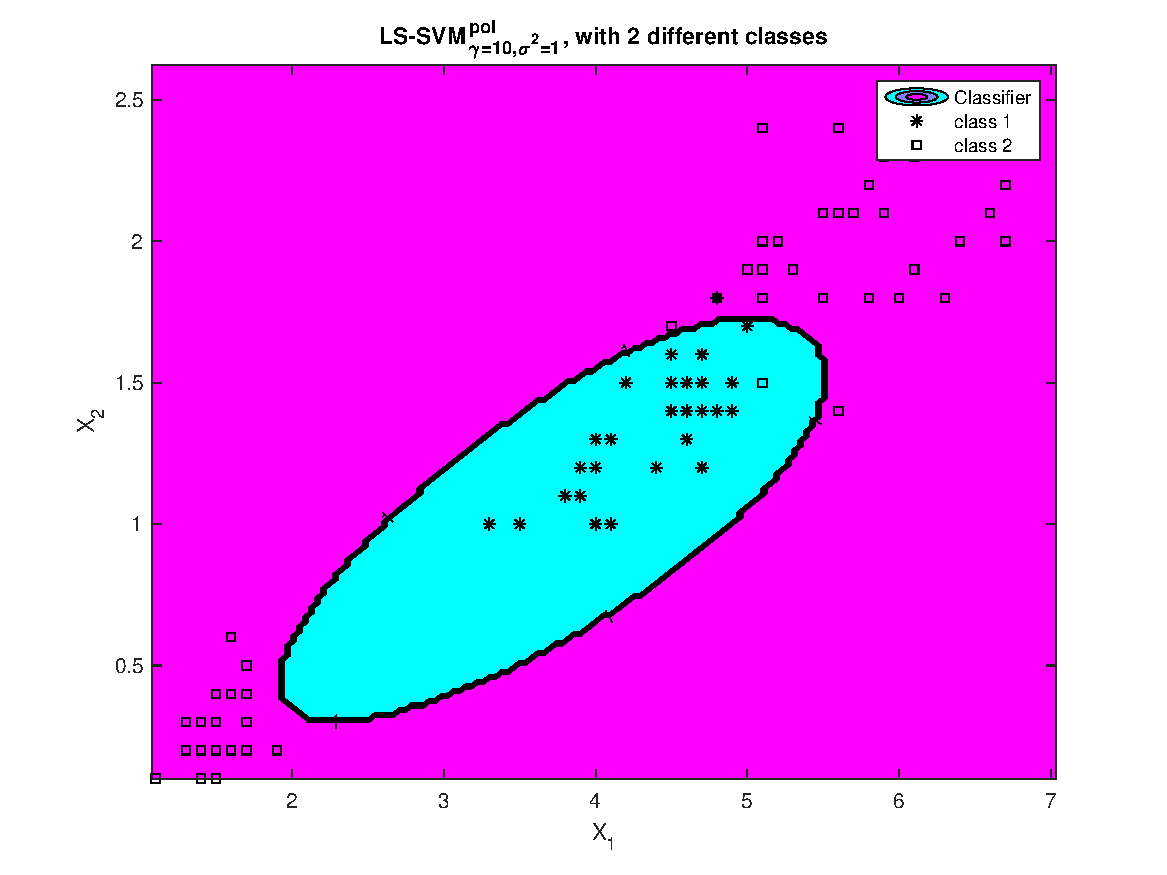
\includegraphics[width=0.3\textwidth]{../src/figures/iris/t=1/3_100}}\qquad
%\\
%\subfloat[$\gamma=0.1,\delta=4,\rho=0.0$]{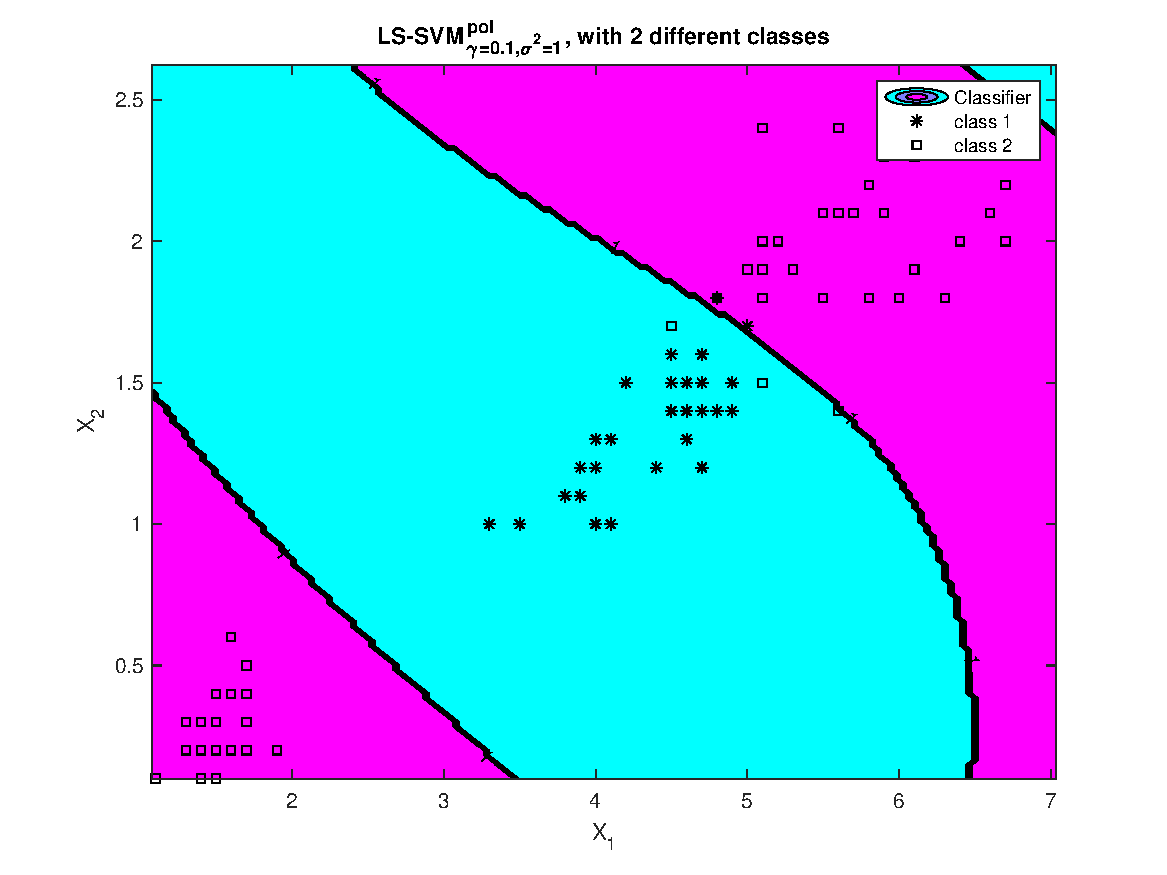
\includegraphics[width=0.3\textwidth]{../src/figures/iris/t=1/4_1}}\qquad
%\subfloat[$\gamma=1.0,\delta=4,\rho=0.0$]{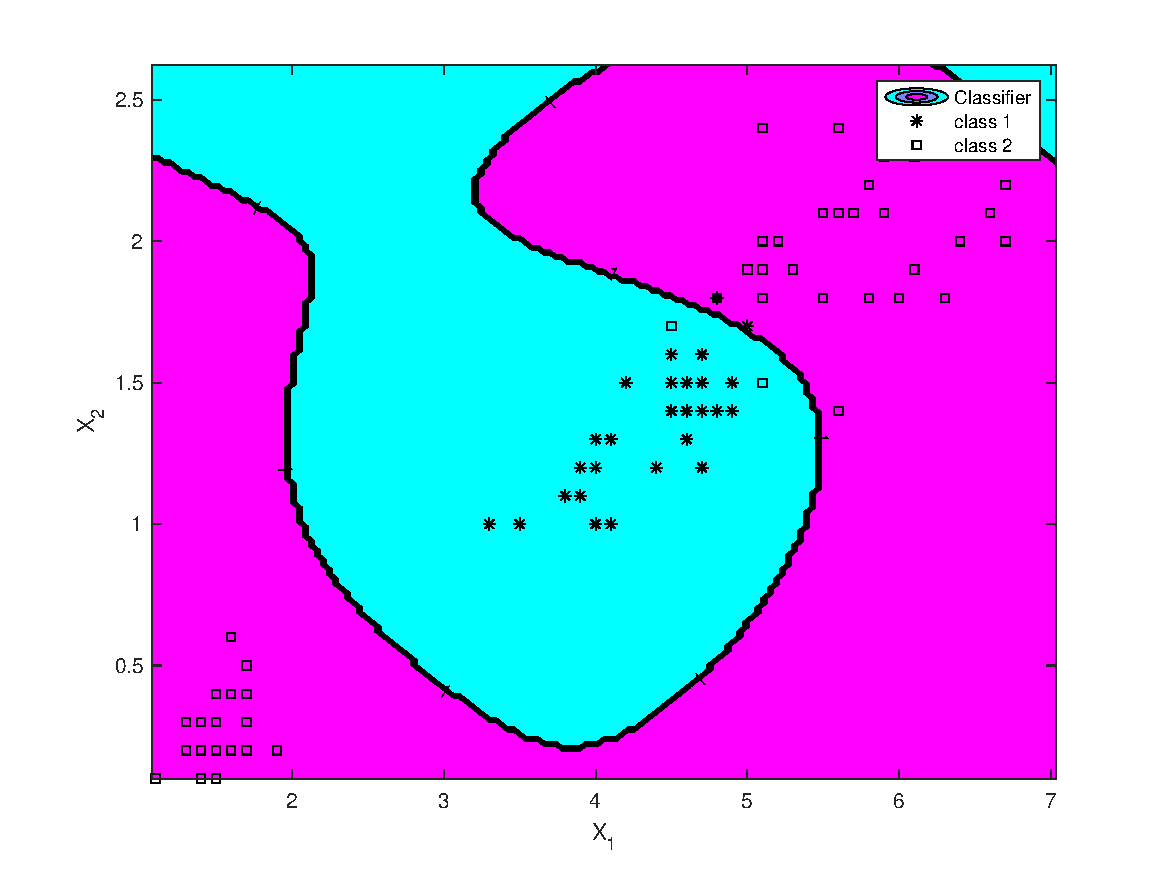
\includegraphics[width=0.3\textwidth]{../src/figures/iris/t=1/4_10}}\qquad
%\subfloat[$\gamma=10.0,\delta=4,\rho=0.0$]{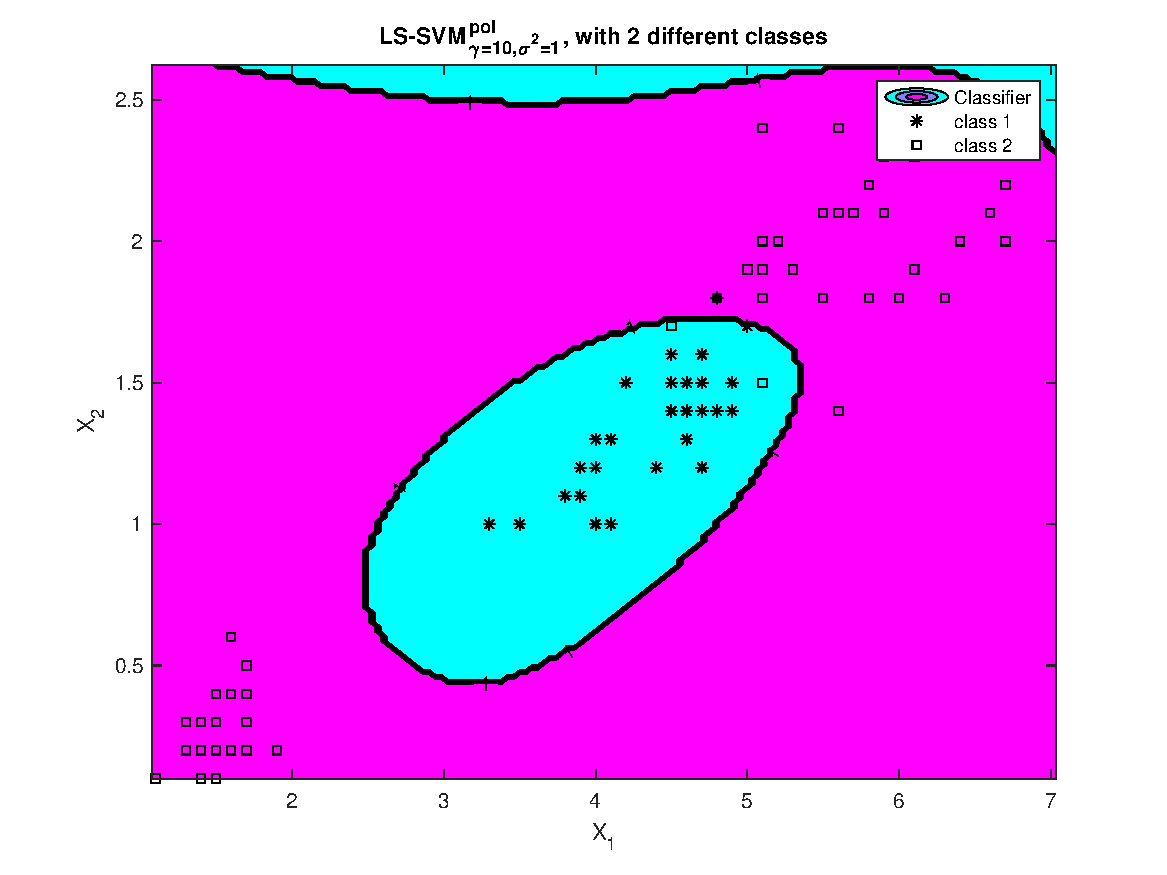
\includegraphics[width=0.3\textwidth]{../src/figures/iris/t=1/4_100}}
%\caption{Visualisation of the results of experiments with polynomial kernels on the iris dataset ($\delta$ is the degree of the polynomial, $\rho$ the misclassification rate on the test set, $t$ is fixed to 1). As the degree of the kernel increases, the misclassification error drops.}
%\end{figure}

\begin{wrapfigure}{l}{0pt}
\hspace*{-0.67cm} 
\centering
\subfloat[$\delta=1,\rho=0.55$]{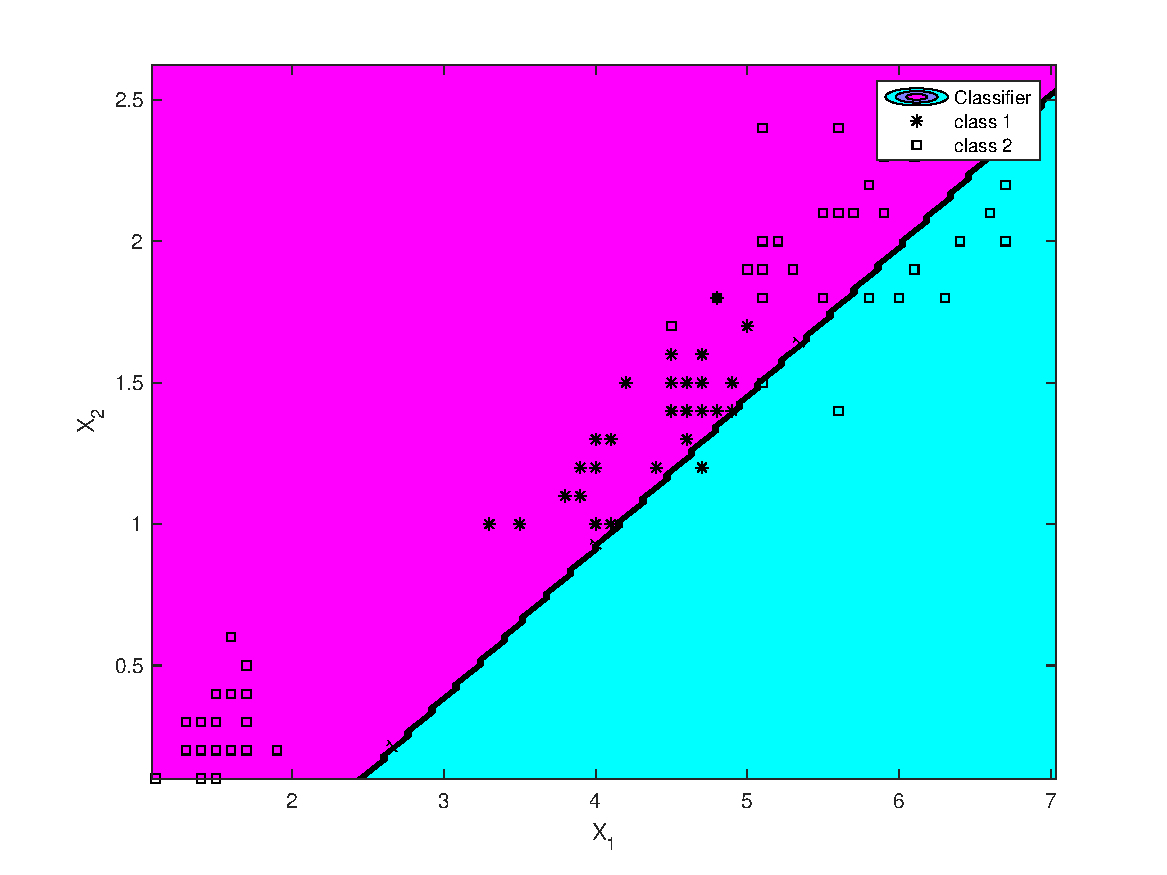
\includegraphics[width=0.25\textwidth]{../src/figures/iris/t=1/1_10}}\quad
\subfloat[$\delta=2,\rho=0.05$]{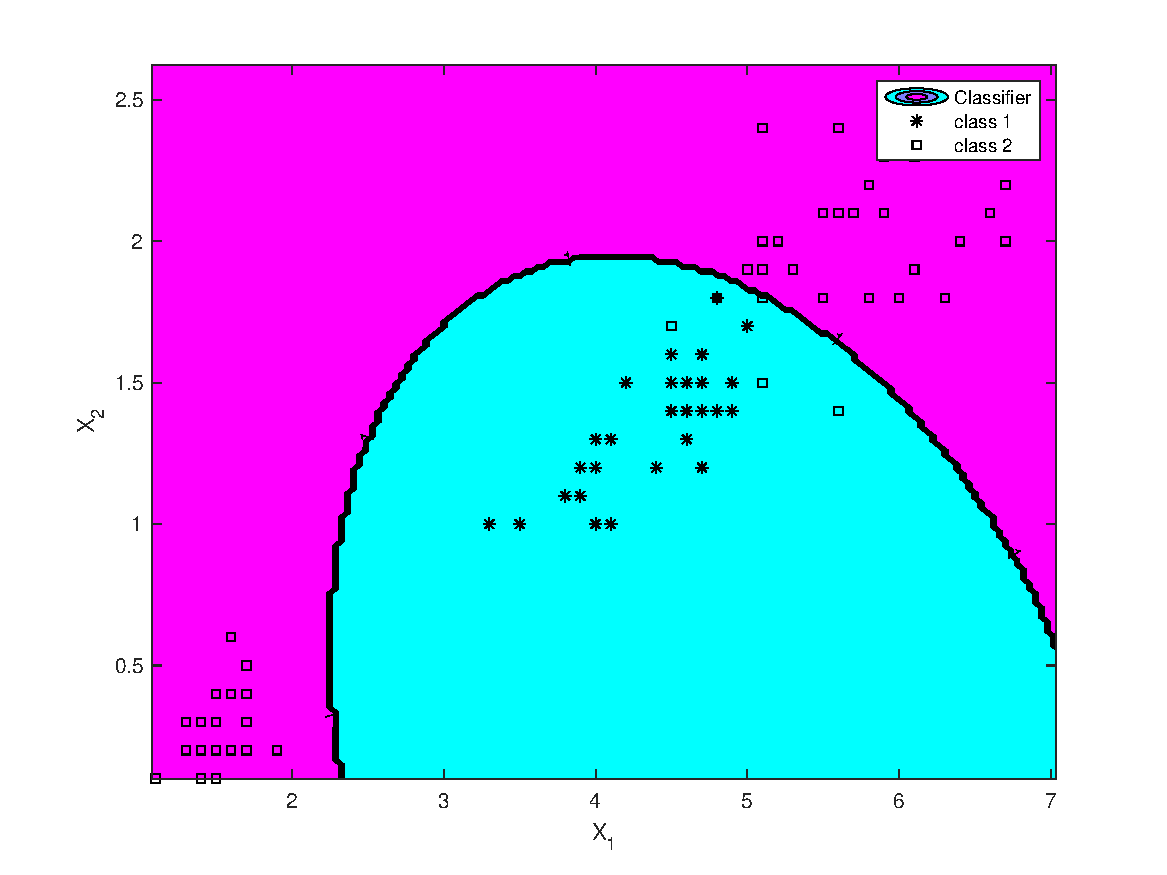
\includegraphics[width=0.25\textwidth]{../src/figures/iris/t=1/2_10}}\quad
\subfloat[$\delta=3,\rho=0.0$]{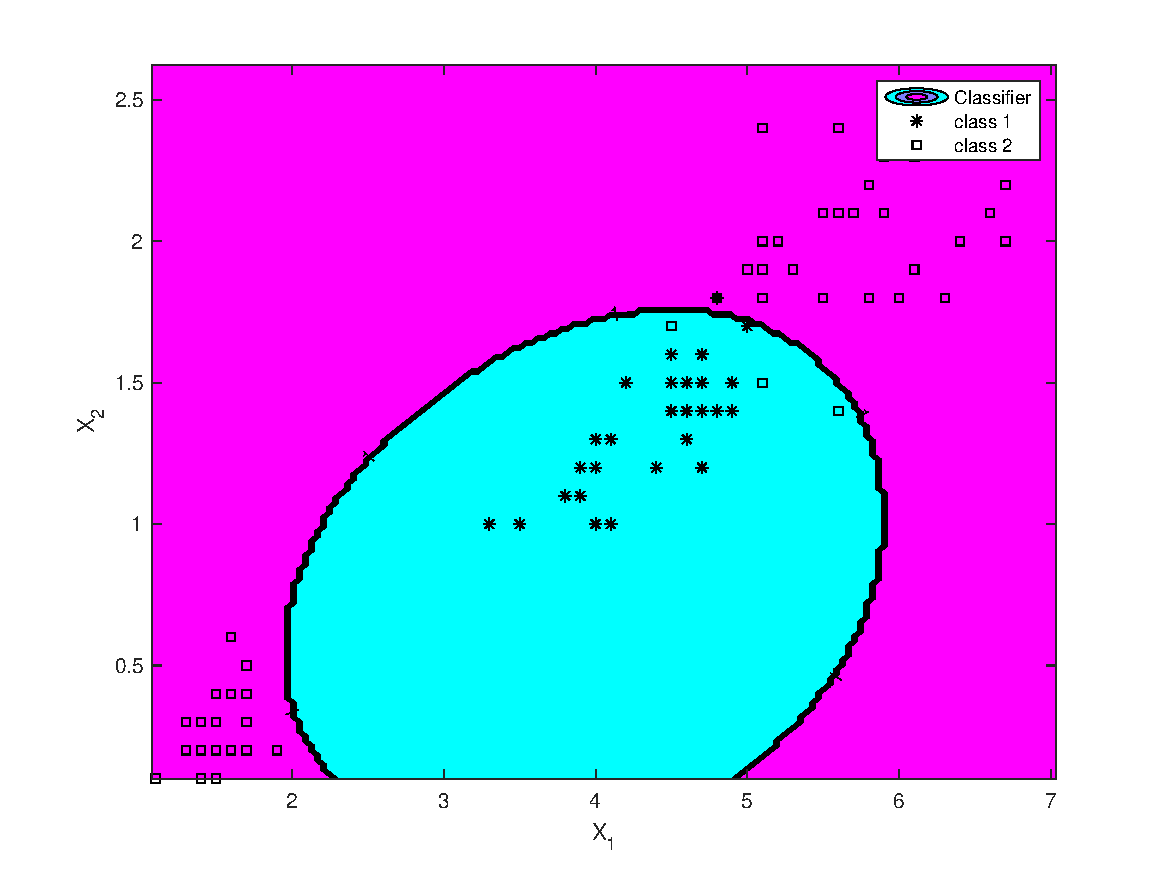
\includegraphics[width=0.25\textwidth]{../src/figures/iris/t=1/3_10}}\quad
\subfloat[$\delta=4,\rho=0.0$]{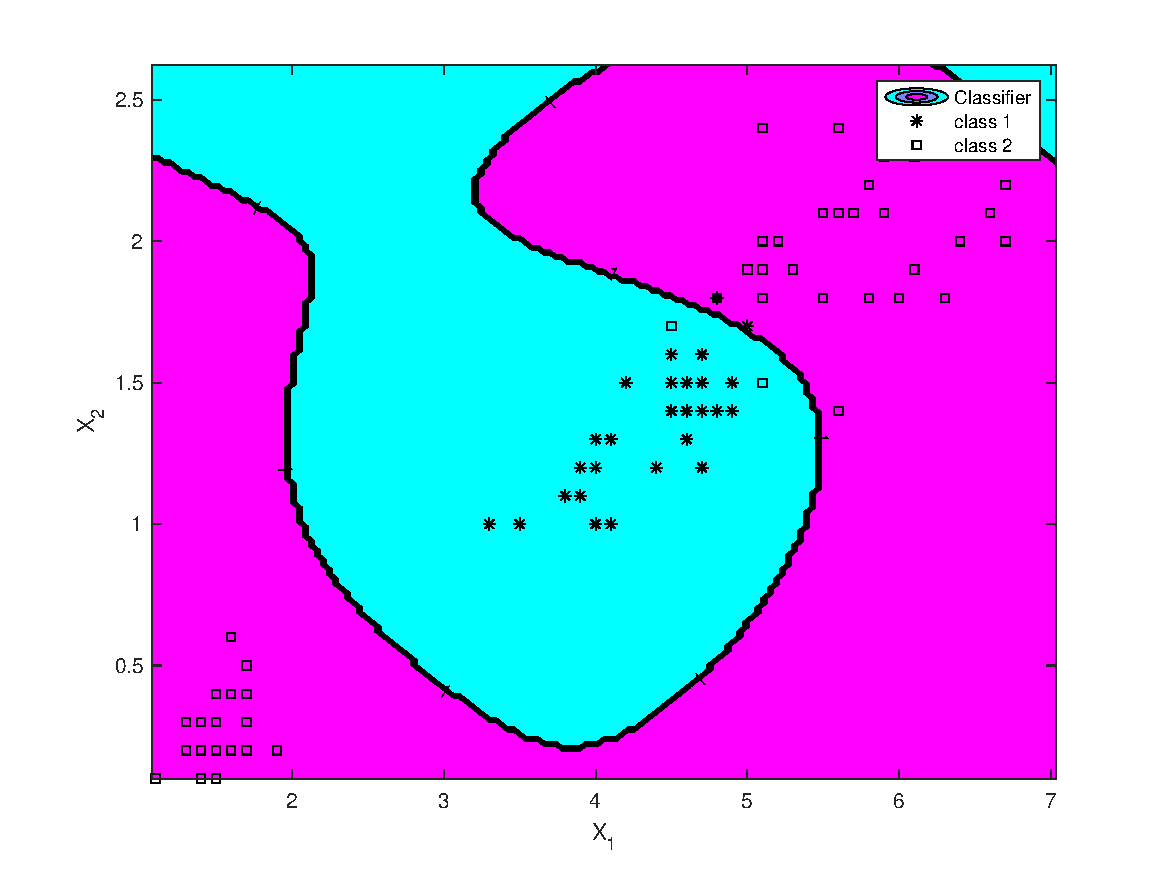
\includegraphics[width=0.25\textwidth]{../src/figures/iris/t=1/4_10}}\quad
\caption{Visualisation of the results of experiments with polynomial kernels on the iris dataset ($\delta$ is the degree of the polynomial, $\rho$ the misclassification rate on the test set, $\tau$ and $\gamma$ are fixed to 1). As the degree of the kernel increases, the misclassification error drops.}
\label{iris}
\end{wrapfigure}

\begingroup
\setlength{\columnsep}{0.75cm}
\setlength{\intextsep}{0.2cm}
\begin{wrapfigure}{r}{0pt}
\centering
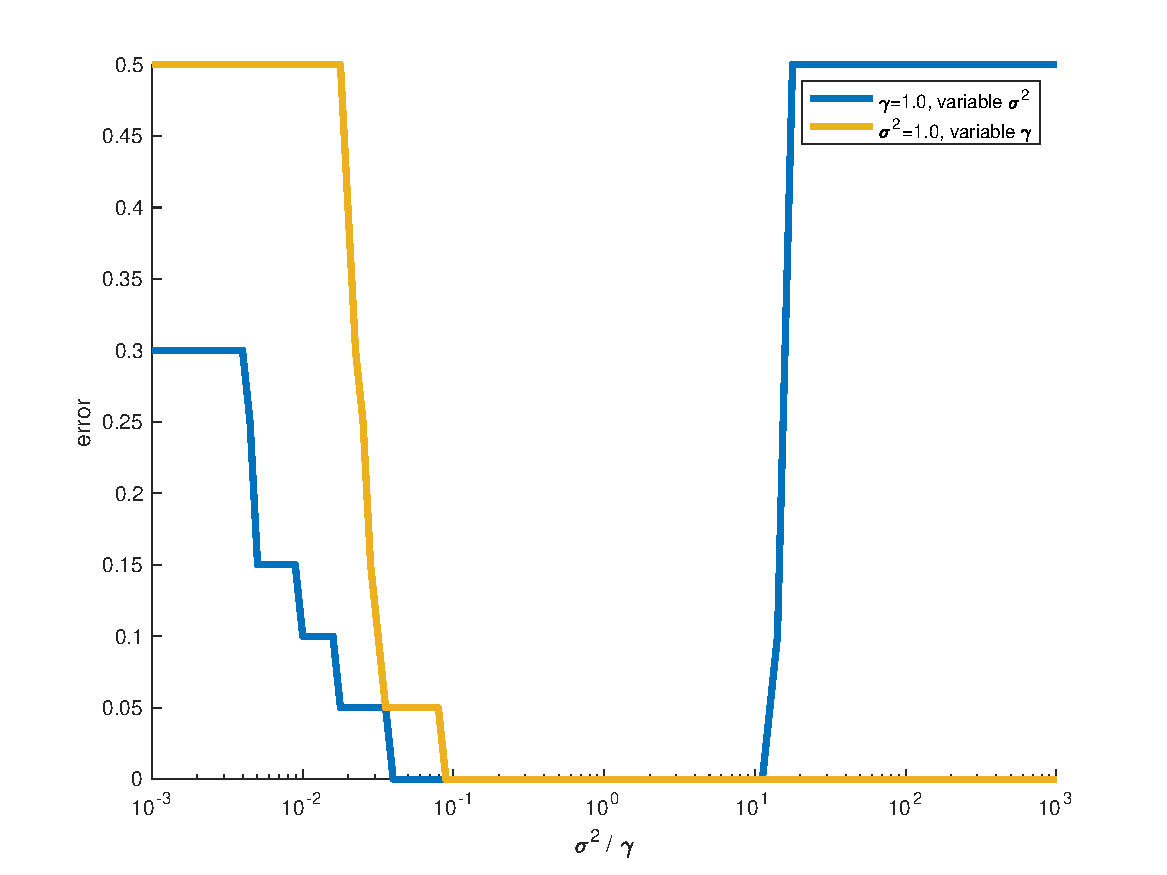
\includegraphics[width=0.45\textwidth]{../src/figures/iris/tuning}
\caption{Performance of various RBF kernels on the iris dataset. The orange curve denotes the performance of the model for varying $\gamma$ and fixed $\sigma^2=1.0$, the blue curve does the opposite ($\gamma=1.0$).}
\label{iris2}
\end{wrapfigure}
\vspace{0.5cm}

\par\noindent  In the case of RBF kernels one can see in figure \ref{iris2} that for a $\gamma$ value of 1 any $\sigma^2$ between 0.1 and 1 performs well. The same interval works for $\gamma$ when $\sigma^2=1$. This corresponds to the results in the sample where the base used in the semilog plot happens to be the natural logarithm (instead of using base 10). For large $\sigma$ values (25 for example) one class may overtake the other one as discussed before. In any case, it should be noted that only a few parameters were tried.

\par\noindent To properly find good parameter values a more systematic approach is in order. The idea is to search through the parameter space and evaluate the results on a validation set rather than on the test set (which should be used for nothing but the evaluation of the finished model). A validation set can be constructed in a few ways the results of which are illustrated in figure \ref{validation}, where error estimates in the parameter space are shown. Random splitting i.e. splitting the input data randomly in a training - and a validation set is a way that isn't particularly robust. An improvement upon it is $k$-fold validation where the input data is randomly split into $k$ folds which are considered as a validation set in turn such that the all input data is used for parameter tuning. When $k=N$ with $N$ the number of input samples this is called leave-one-out cross-validation. 

\endgroup

\par To some extent deciding what $k$ value to use parallels previous discussions about other parameters since there's a bias-variance tradeoff ; while larger $k$ values should provide a better estimate of the error they also suffer from higher variance as the result depends more on how representative the input data is. This becomes more important when the number of input data is small. Finally, $k$ shouldn't be too small (such that the training sets remain large enough), it should preferably be a divisor of $N$ (though this is not of primary importance) and if computational expense is an issue it cannot be large as many models need to be generated in that case.

\par Automated tuning uses these validation methods in conjunction with a search procedure to find useful combinations of parameters. This search strategy has to deal with a non-convex problem and can be a simple grid search (performing validation for every combination of parameters specified by a grid partitioning the parameter space) or the Nelder-Mead method which aims to find the minimum of a function without needing its derivative. The latter considers a simplex and updates it iteratively until the minimum is found. It tends to execute faster than grid search especially when the number of parameters is high, though one could also consider a variant of grid search that starts with a grid of limited granularity until it finds a promising region in the parameter space on which grid search is performed again.

\par In the LS-SVM toolbox a technique called \textit{coupled simulated annealing} is used. This is a global optimisation technique which couples together several simulated annealing processes (inspired by coupled local minimisers' effectiveness compared to multi-start gradient descent optimisation). Its output is provided to either a grid search - or a Nelder-Mead algorithm. Results are the following :

\begin{table}[h]
\centering
\begin{tabular}{c|ccc}
\textit{Method} & \textit{Average} & \textit{STD} & \textit{Total runtime} \\
\hline
Grid search & XXX & XXX & XXX\\
Nelder-Mead & XXX & XXX & XXX\\
\end{tabular}
\caption{Results of automated tuning strategies (average over ten runs).}
\label{automatedtuning}
\end{table}

Clearly the results are quite varied. A histogram of the results gives a more complete picture :

\begin{figure}[h]
\includegraphics[width=0.5\textwidth]{../src/figures/iris/tuninghistogram}
\caption{Results of automated tuning strategies in a histogram format.}
\label{automatedtuninghistogram}
\end{figure}

Cleary (ADD DESCRIPTION HERE)

\begin{wrapfigure}{r}{.45\textwidth}
\begin{minipage}{\linewidth}
    \centering\captionsetup[subfigure]{justification=centering}
    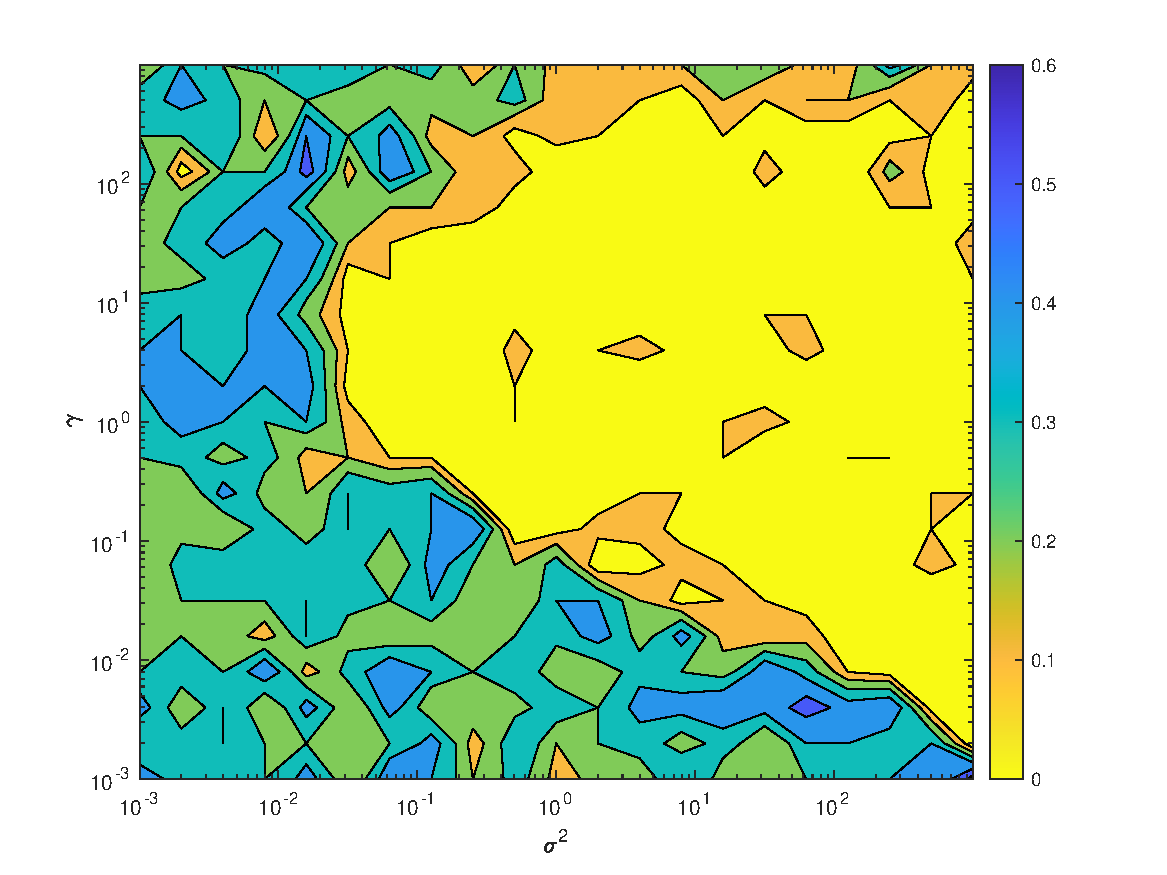
\includegraphics[width=\linewidth]{../src/figures/iris/validation_1}
    \caption*{(a) Random split validation.}
    \label{fig:5a}\par\vfill
    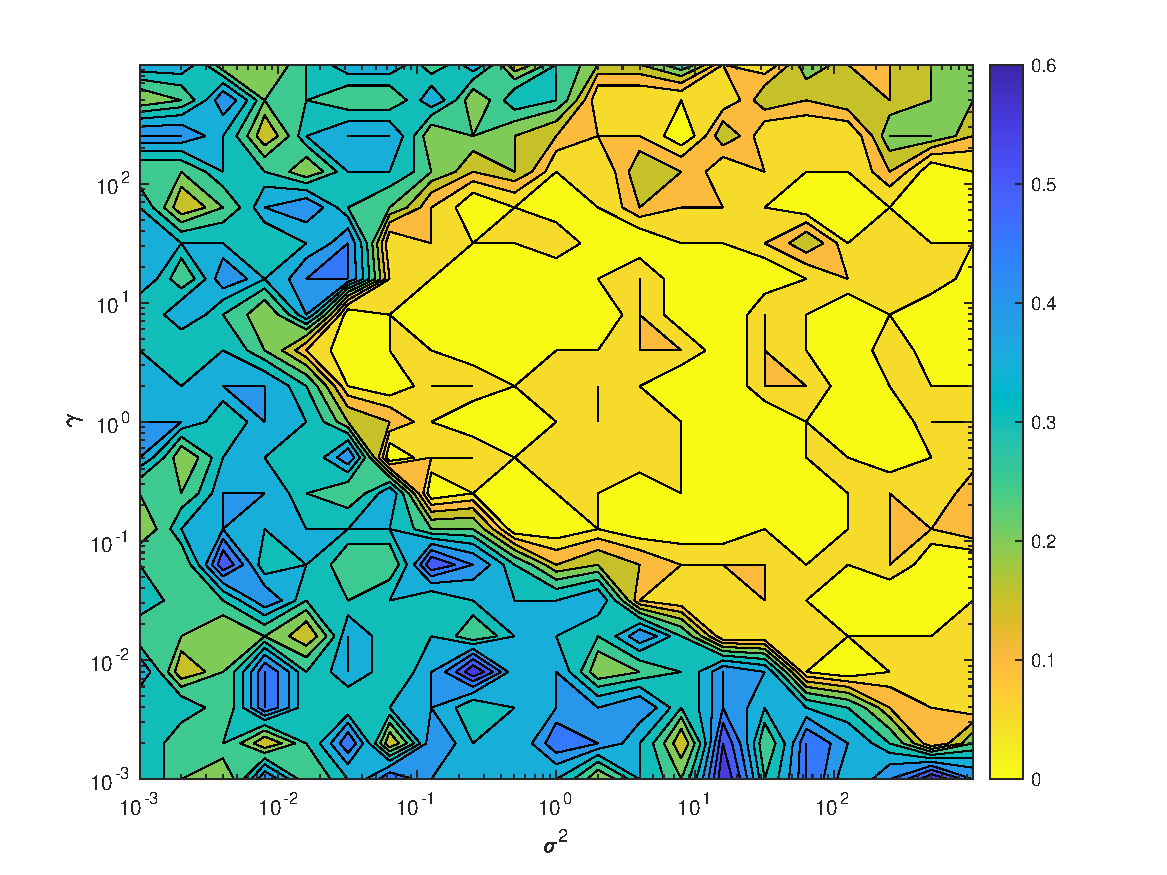
\includegraphics[width=\linewidth]{../src/figures/iris/validation_2}
    \caption*{(b) $k$-fold validation ($k=10$).}
    \label{fig:5b}
    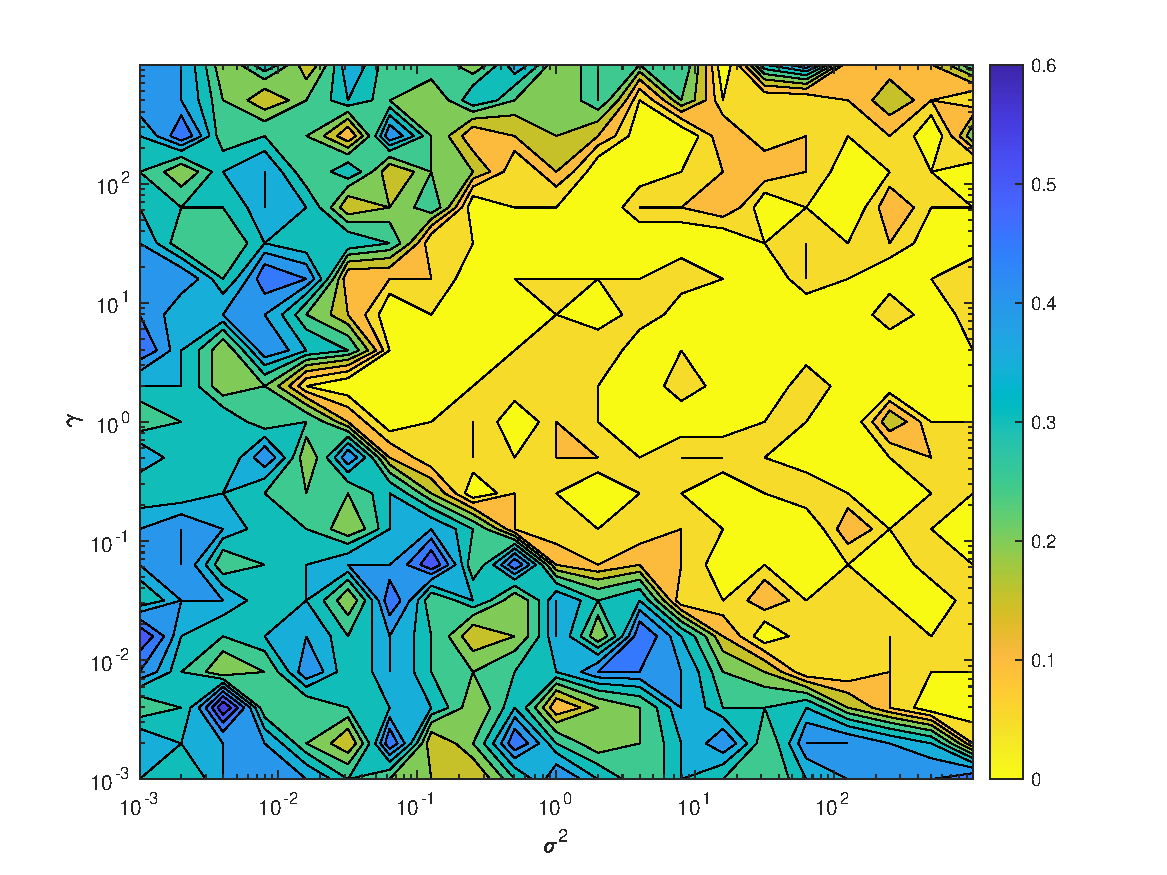
\includegraphics[width=\linewidth]{../src/figures/iris/validation_3}
    \caption*{(c) Leave-one-out validation.}
    \label{fig:5c}
\end{minipage}
\caption{Grid search in conjunction with various validation techniques. The results differ and the results for the random split strategy varies between runs. $k$-fold crossvalidation appears to be a better approximation of the error but may generalise less well. Reasonable parameters lie in the yellow zone where the error reaches a maximum of about 10\%. A small bandwidth of between say, 0.1 and 1.0 and a regularization constant of 1.0 seems reasonable.}
\label{validation}
\end{wrapfigure}

\fakesubsection{Ripley dataset}{}

\fakesubsection{Wisconsin breast cancer dataset}{}

\fakesubsection{Diabetes dataset}{}


